\documentclass[11pt, handout, aspectratio=169]{beamer}
\usepackage{style/jrc-beamer}

% uncomment to print two slides per page
% \handout

\usepackage{amssymb}
\usepackage{pifont}
\usepackage{pgf}

\usepackage{booktabs}
\usepackage{multirow}

\usepackage{tikz}
\usetikzlibrary{arrows, decorations.markings}
\tikzstyle{every picture}+=[remember picture]

\usepackage{acronym}
\usepackage{xcolor}

\hypersetup{colorlinks,
citecolor=blue,
linkcolor=.,
menucolor=white,
filecolor=pink,   
anchorcolor=yellow
}

% RIN Red Color
\definecolor{rinred}{RGB}{161,7,40}
\definecolor{darkg}{RGB}{75, 75, 75}
\definecolor{lightg}{RGB}{230, 230, 230}
\definecolor{lightgreen}{RGB}{226, 240, 217}
\definecolor{azure}{RGB}{232,232,255}

% for code listing
%% \usepackage{minted}
\usepackage{listings}
\usepackage{adjustbox}
\usepackage{lipsum}
\usepackage{courier}

%% \lstset{basicstyle=\footnotesize\ttfamily,breaklines=true}
%% \lstset{framextopmargin=50pt}
\lstset{
  language=python,
  basicstyle=\footnotesize\ttfamily,
  breaklines=true,
  keepspaces=true,
  backgroundcolor=\color{lightgreen},
  frame=single,
  framerule=0pt,  
  moredelim=**[is][\color{red}]{@}{@},
  %% framextopmargin=3ex,
  %% framexbottommargin=3ex,
  %% framexleftmargin=1em,
  %% xleftmargin=\dimexpr 1em+3pt\relax,
  %% linewidth=\dimexpr \linewidth-3pt\relax
}
%% \lstset{framextopmargin=50pt,frame=bottomline}
%% \lstset{escapeinside={<@}{@>}}

\setbeamerfont{outline}{size={\fontsize{15}{16}}, series=\bfseries}
\setbeamerfont{link}{size={\fontsize{11}{12}}, series=\bfseries}

\def\graytextbox#1{
\begin{pgfpicture}
	\pgfsetfillcolor{lightg}
	\pgfsetstrokecolor{black}
	\pgfrect[fillstroke]{\pgfxy(0,0)}{\pgfxy(8.7, 0.8)}
	\begin{pgftranslate}{\pgfxy(4.35, 0.4)}
		\pgftext[center]{\usebeamerfont{outline}\usebeamercolor[fg]{title}#1}
	\end{pgftranslate}
\end{pgfpicture}
}

\def\bluetextbox#1{
\begin{pgfpicture}
	\pgfsetfillcolor{azure}
	\pgfsetstrokecolor{textcolor}
	\pgfrect[fillstroke]{\pgfxy(0,0)}{\pgfxy(8.7, 0.8)}
	\begin{pgftranslate}{\pgfxy(4.35, 0.4)}
		\pgftext[center]{\usebeamerfont{outline}\usebeamercolor[fg]{normal text}#1}
	\end{pgftranslate}
\end{pgfpicture}
}

\def\greenbox#1{
\setbeamercolor{lightbox}{fg=textcolor, bg=lightgreen}
\begin{beamercolorbox}[wd=\textwidth,rounded=true]{lightbox}
{#1}
\end{beamercolorbox}	
}

\def\bluebox#1{
\setbeamercolor{lightbox}{fg=textcolor, bg=azure}
\begin{beamercolorbox}[wd=\textwidth,rounded=true]{lightbox}
{#1}
\end{beamercolorbox}	
}

\def\redbox#1{
\setbeamercolor{lightbox}{fg=white, bg=rinred}
\begin{beamercolorbox}[wd=\textwidth,rounded=true]{lightbox}
{#1}
\end{beamercolorbox}	
}

\def\greeneq#1{
$\tikz[baseline]{
            \node[fill=lightgreen,anchor=base]
            {$#1$};}$
}

%%%%%%%%%%%%%%%%%%%%%%%%%%%%%%%%%%%%%%%%%%%%%%%%%%%%%%%%%%%%%%%%%%%%%%%%%%%%%%%%%%
\TitlePageType{1} % From 1 to 3
\shrinktitle

% Copyright notice
\CopyrightInfo{Slide xx: element concerned, source: e.g. Fotolia.com; Slide xx: element concerned, source: e.g. iStock.com}

\title{pyjeo}

\subtitle{an open source image processing library \\
  in Python}
% \subtitle{}   - It is also possible to add a subtitle
\author{Pieter Kempeneers\\
\textbf{Matera, Italy}}
\date{13 June 2022}
% \nodate

\begin{document}


%%%%%%%%%%%%%%%%%%%%%%%%%%%%%%%%%%%%%%%%%%%%%%%%%%%%%%%%%%%%%%%%%%%%%%%%%%%%%%%%%%%%%%%%%%%%%%%%%%%%
%																						Title Frame		  																			 %		
%%%%%%%%%%%%%%%%%%%%%%%%%%%%%%%%%%%%%%%%%%%%%%%%%%%%%%%%%%%%%%%%%%%%%%%%%%%%%%%%%%%%%%%%%%%%%%%%%%%%

\begin{frame}
	\maketitle	
\end{frame}

%%%%%%%%%%%%%%%%%%%%%%%%%%%%%%%%%%%%%%%%%%%%%%%%%%%%%%%%%%%%%%%%%%%%%%%%%%%%%%%%%%%%%%%%%%%%%%%%%%%%
%																						Installation and usage																 %		
%%%%%%%%%%%%%%%%%%%%%%%%%%%%%%%%%%%%%%%%%%%%%%%%%%%%%%%%%%%%%%%%%%%%%%%%%%%%%%%%%%%%%%%%%%%%%%%%%%%%

\begin{frame}[fragile]
  \frametitle{Installation}
  \usebeamerfont{normal}
  \begin{itemize}
  \item source code available in \href{https://github.com/ec-jrc/jeolib-pyjeo}{github}
  \item dependencies (C/C++ code):
    \begin{itemize}
    \item \href{https://github.com/ec-jrc/jeolib-miallib}{miallib}
    \item \href{https://github.com/ec-jrc/jeolib-jiplib}{jiplib} (derived from pktools with Python interface)
    \end{itemize}
  \end{itemize}
\end{frame}

%%%%%%%%%%%%%%%%%%%%%%%%%%%%%%%%%%%%%%%%%%%%%%%%%%%%%%%%%%%%%%%%%%%%%%%%%%%%%%%%%%%%%%%%%%%%%%%%%%%%
%																						Docker environment    																 %		
%%%%%%%%%%%%%%%%%%%%%%%%%%%%%%%%%%%%%%%%%%%%%%%%%%%%%%%%%%%%%%%%%%%%%%%%%%%%%%%%%%%%%%%%%%%%%%%%%%%%

\begin{frame}[fragile]
  \frametitle{Installation}
  \usebeamerfont{normal}
  

  Build docker image using \href{https://github.com/ec-jrc/jeolib-pyjeo/blob/master/docker/Dockerfile_deb10_pyjeo_public}{Dockerfile} (based on a debian11 image):

  \begin{lstlisting}{bash}
    docker build -t deb11_pyjeo_public:0.1.8 -f Dockerfile_deb11_pyjeo_public .
  \end{lstlisting}

  Run pyjeo in Docker container:

  \begin{lstlisting}{bash}
    docker run --rm deb11_pyjeo_public:0.1.8 python3 -c "import pyjeo as pj; jim = pj.Jim(ncol = 10, nrow = 10, nband = 3); print(jim.properties.nrOfBand())"   
  \end{lstlisting}
\end{frame}

%%%%%%%%%%%%%%%%%%%%%%%%%%%%%%%%%%%%%%%%%%%%%%%%%%%%%%%%%%%%%%%%%%%%%%%%%%%%%%%%%%%%%%%%%%%%%%%%%%%%
%																						Functions and Methods                                  %
%%%%%%%%%%%%%%%%%%%%%%%%%%%%%%%%%%%%%%%%%%%%%%%%%%%%%%%%%%%%%%%%%%%%%%%%%%%%%%%%%%%%%%%%%%%%%%%%%%%%

\begin{frame}[fragile]
  \frametitle{Methods}
  \usebeamerfont{normal}
  
  \begin{itemize}
  \item Methods directly operate on objects, i.e., instances of a class
  \item Methods can change objects in-place (overwrite input)
  \item No object is returned
  \end{itemize}

  \begin{lstlisting}{python}
    jim.geometry.cropBand(0)
  \end{lstlisting}
  jim has been cropped in-place and \lstinline{None} is returned

\end{frame}

\begin{frame}[fragile]
  \frametitle{Functions}
  \usebeamerfont{normal}
  \begin{itemize}
  \item Functions that operate on objects must have the objects passed as arguments
  \item Functions leave their arguments unaltered
  \item A new object (newobject) is returned
  \end{itemize}
  
  \begin{lstlisting}{python}
    jim_cropped = pj.geometry.cropBand(jim, 0)
  \end{lstlisting}
  jim is unaltered and a \lstinline{Jim} object is returned
\end{frame}

%%%%%%%%%%%%%%%%%%%%%%%%%%%%%%%%%%%%%%%%%%%%%%%%%%%%%%%%%%%%%%%%%%%%%%%%%%%%%%%%%%%%%%%%%%%%%%%%%%%%
%																						Documentation                                          %
%%%%%%%%%%%%%%%%%%%%%%%%%%%%%%%%%%%%%%%%%%%%%%%%%%%%%%%%%%%%%%%%%%%%%%%%%%%%%%%%%%%%%%%%%%%%%%%%%%%%

\begin{frame}[fragile]
  \frametitle{Documentation}
  \usebeamerfont{normal}
  \vspace{7mm}

  The documentation is \href{https://jeodpp.jrc.ec.europa.eu/services/processing/pyjeohelp/index.html}{online} and can be accessed outside the Commission.
  \vspace{7mm}
	\begin{center}
		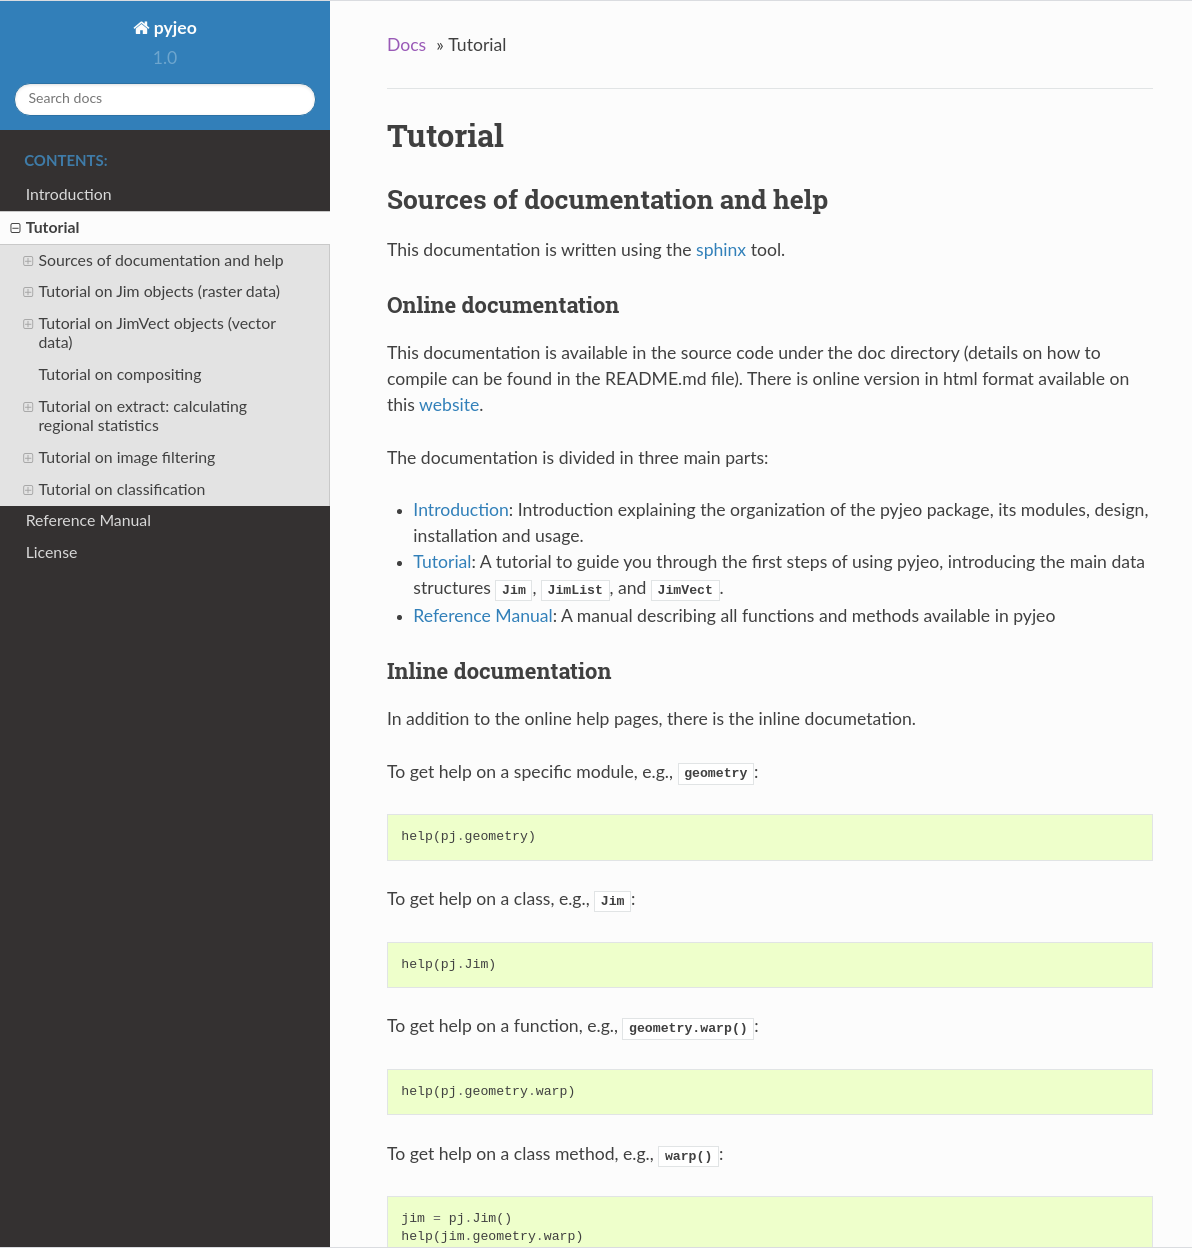
\includegraphics[height=0.7 \textheight]{figures/documentation}
	\end{center}
\end{frame}

\begin{frame}[fragile]
  \frametitle{Documentation (inline)}
  \usebeamerfont{normal}
  \begin{itemize}
  \item To get help on a specific module, e.g., geometry:
    \begin{lstlisting}{python}
      help(pj.geometry)
    \end{lstlisting}
  \item To get help on a class, e.g., Jim:
    \begin{lstlisting}{python}
      help(pj.Jim)
    \end{lstlisting}
  \item To get help on a function, e.g., \lstinline{geometry.warp()}:
    \begin{lstlisting}{python}
      help(pj.geometry.warp)
    \end{lstlisting}
  \end{itemize}

  \vspace{2mm}
  Check also the online \href{https://jeodpp.jrc.ec.europa.eu/services/processing/pyjeohelp/2_tutorial.html}{tutorial}.
  \vspace{2mm}
\end{frame}

%%%%%%%%%%%%%%%%%%%%%%%%%%%%%%%%%%%%%%%%%%%%%%%%%%%%%%%%%%%%%%%%%%%%%%%%%%%%%%%%%%%%%%%%%%%%%%%%%%%%
%															Data model: Jim and JimVect                                          %
%%%%%%%%%%%%%%%%%%%%%%%%%%%%%%%%%%%%%%%%%%%%%%%%%%%%%%%%%%%%%%%%%%%%%%%%%%%%%%%%%%%%%%%%%%%%%%%%%%%%

\begin{frame}[fragile]
  \frametitle{Data model: Jim}
  \usebeamerfont{normal}

  \vspace{7mm}
  \textbf{Jim: pyjeo object for multi-band 3D raster data}

	\begin{center}
		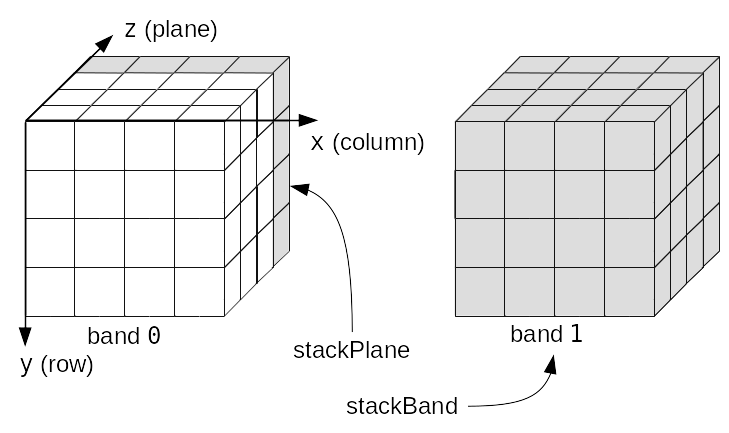
\includegraphics[width=0.65\textwidth]{figures/cube}
	\end{center}
\end{frame}

\begin{frame}[fragile]
  \frametitle{Data model: Jim}
  \usebeamerfont{normal}
  \begin{itemize}
  \item Each band represents a 3D contiguous array in memory: space (2) + plane (1)
  \item Planes are typically used for temporal/spectral/volumetric data
  \item data cube is defined in a single spatial reference system (geotransform and projection)
  \end{itemize}
\end{frame}

\begin{frame}[fragile]
  \frametitle{Data model: JimVect}
  \usebeamerfont{normal}
  \vspace{7mm}
  \textbf{JimVect: pyjeo object for vector data}
  \vspace{7mm}
  \begin{itemize}
  \item References to file path that represents a vector
  \item File format must be supported by GDAL
  \item File can be virtual (in memory only)
  \end{itemize}
\end{frame}

%%%%%%%%%%%%%%%%%%%%%%%%%%%%%%%%%%%%%%%%%%%%%%%%%%%%%%%%%%%%%%%%%%%%%%%%%%%%%%%%%%%%%%%%%%%%%%%%%%%%
%															Reading/writing geospatial data                                      %
%%%%%%%%%%%%%%%%%%%%%%%%%%%%%%%%%%%%%%%%%%%%%%%%%%%%%%%%%%%%%%%%%%%%%%%%%%%%%%%%%%%%%%%%%%%%%%%%%%%%

\begin{frame}[fragile]
  \frametitle{Reading/writing geospatial data}
  \usebeamerfont{normal}
  As a default, a multi-band raster file is read as a single plane multi-band Jim object.
  \begin{lstlisting}{python}
    jim = pj.Jim('/path/to/raster.tif')
  \end{lstlisting}

	\begin{center}
		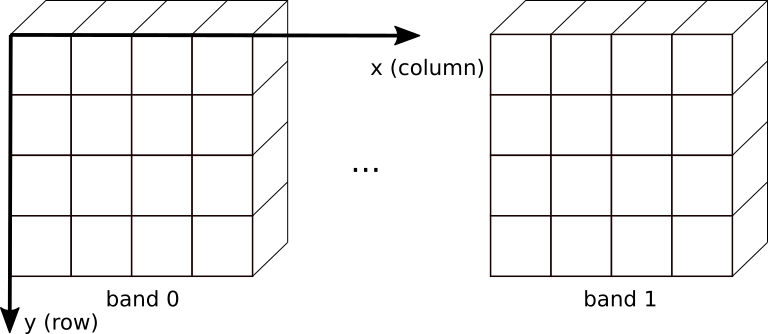
\includegraphics[scale=0.4]{figures/multiband}
	\end{center}
\end{frame}

\begin{frame}[fragile]
  \frametitle{Reading/writing geospatial data}
  \vspace{5mm}
  \usebeamerfont{normal}
  To open the image as a 3D multi-plane Jim object, use the \lstinline{band2plane} argument
  \begin{lstlisting}{python}
    jim = pj.Jim('/path/to/raster.tif', band2plane = True)
  \end{lstlisting}

	\begin{center}
		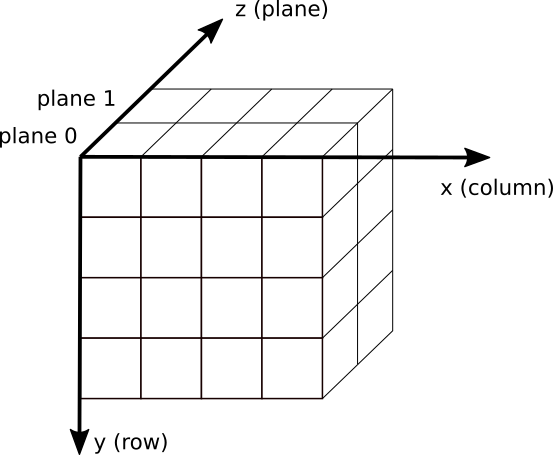
\includegraphics[scale=0.4]{figures/multiplane}
	\end{center}
\end{frame}

\begin{frame}[fragile]
  \frametitle{Converting bands and planes}
  \usebeamerfont{normal}
	\begin{center}
		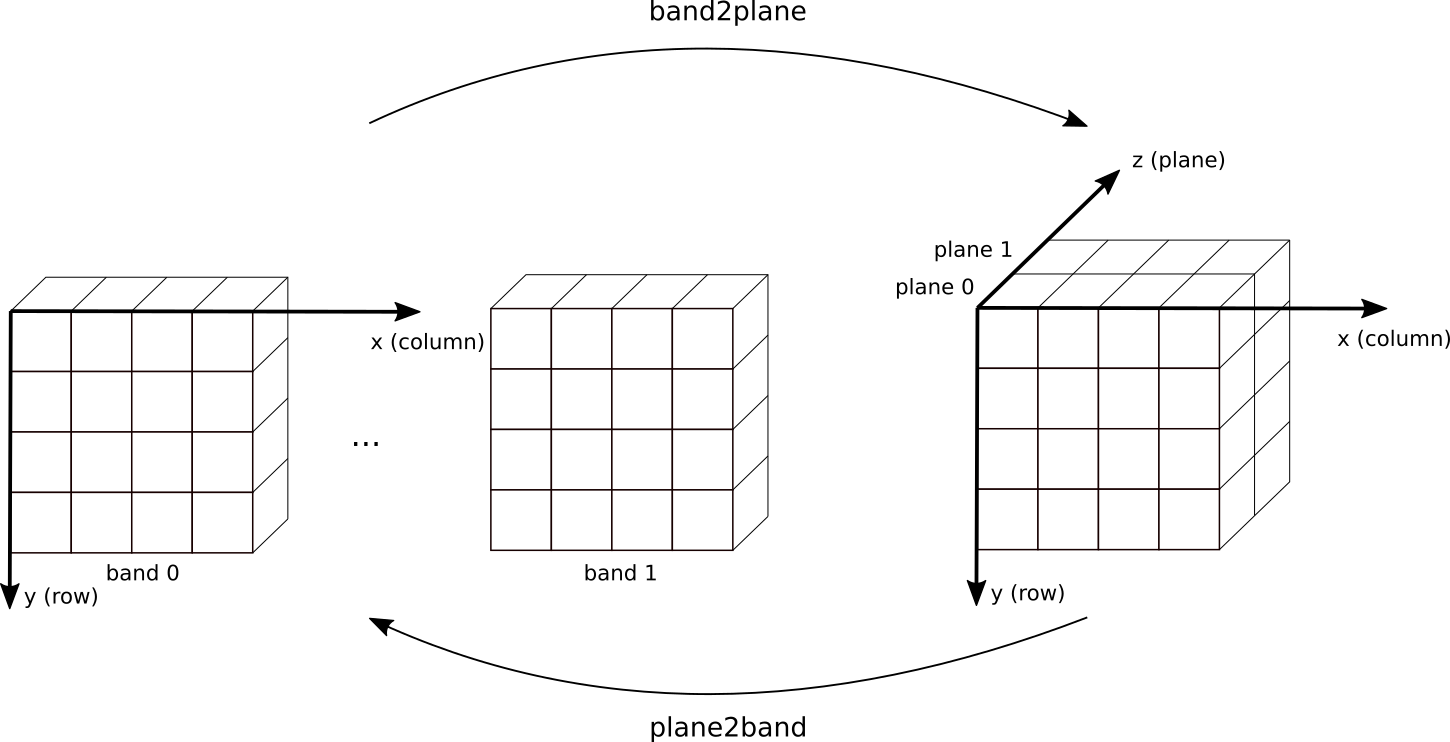
\includegraphics[scale=0.25]{figures/band2plane}
	\end{center}
\end{frame}

%%%%%%%%%%%%%%%%%%%%%%%%%%%%%%%%%%%%%%%%%%%%%%%%%%%%%%%%%%%%%%%%%%%%%%%%%%%%%%%%%%%%%%%%%%%%%%%%%%%%
%															Bridging to third party libraries                                    %
%%%%%%%%%%%%%%%%%%%%%%%%%%%%%%%%%%%%%%%%%%%%%%%%%%%%%%%%%%%%%%%%%%%%%%%%%%%%%%%%%%%%%%%%%%%%%%%%%%%%

\begin{frame}[fragile]
  \frametitle{Bridging Jim to third party libraries}
  \usebeamerfont{normal}
  \vspace{7mm}
  pyjeo Jim objects can be converted to:
  \begin{itemize}
  \item \href{https://numpy.org}{Numpy} array objects
  \item \href{http://xarray.pydata.org}{xarray} objects)
  \end{itemize}
  Conversion can be performed with memory copy:
  \begin{lstlisting}{python}
    jim = pj.np2jim(nparray)
    nparray = pj.jim2np(jim)
  \end{lstlisting}
  Conversion can be performed without memory copy:
  \begin{lstlisting}{python}
    jim.np()[:] = nparray
    nparray = jim.np() #careful!
  \end{lstlisting}
  \bluebox{The Jim object should remain the owner of the data and the referenced Numpy array object cannot be altered in shape and data type nor destroyed.}
\end{frame}

\begin{frame}[fragile]
  \frametitle{Bridging Jim to third party libraries}
  \usebeamerfont{normal}
  \vspace{7mm}
  \bluebox{Numpy arrays do not have an attribute for a spatial reference system.}
  \vspace{7mm}
  \begin{lstlisting}{python}
    jim = pj.np2jim(nparray)
    jim.properties.setGeoTransform([a,b,c,d,e,f)
      jim.properties.setProjection('epsg:3035')
  \end{lstlisting}
  where the geotransform array \lstinline{[a,b,c,d,e,f]} can also be copied from another Jim object.
  \vspace{7mm}
  \begin{lstlisting}{python}
    gt = jim0.properties.getGeoTransform()
    proj = jim0.properties.getProjection()
  \end{lstlisting}
\end{frame}

\begin{frame}[fragile]
  \frametitle{Bridging Jim to third party libraries}
  Example: in-place Gaussian filtering using ndimage
  \usebeamerfont{normal}
  \vspace{7mm}
  \begin{lstlisting}{python}
    from scipy import ndimage
    jim.np()[:] = ndimage.gaussian_filter(jim.np(), 2)
  \end{lstlisting}
  \vspace{7mm}
\end{frame}

\begin{frame}[fragile]
  \frametitle{Bridging JimVect to third party libraries}
  \usebeamerfont{normal}
  \vspace{7mm}
  pyjeo JimVect objects can be converted to:
  \begin{itemize}
  \item Python dictionaries
  \item \href{https://numpy.org}{Numpy} array objects
  \item \href{https://pandas.pydata.org/pandas-docs/stable/index.html}{pandas} objects
  \item \href{https://geopandas.org/}{geopandas} objects
  \end{itemize}
  \vspace{7mm}
  \begin{lstlisting}{python}
    dictobject = v.dict()
  \end{lstlisting}
  \vspace{7mm}
  \begin{lstlisting}{python}
    nparray = v.np()
  \end{lstlisting}
\end{frame}

\begin{frame}[fragile]
  \frametitle{Bridging JimVect to third party libraries}
  \usebeamerfont{normal}
  \textbf{Convert JimVect to pandas object}
  \begin{lstlisting}{python}
    import pandas as pd
    panda_object = pd.DataFrame(v.dict())
  \end{lstlisting}
  \textbf{Convert JimVect to geopandas object}
  \begin{lstlisting}{python}
    import geopandas as gpd
    v = pj.JimVect('vector.shp')
    #convert to GeoJSON in memory
    vjson = pj.JimVect(v,output='/vsimem/pj.json', oformat = 'GeoJSON')
    vjson.io.close()
    #create geopandas dataframe from GeoJSON file in memory
    gdf = gpd.read_file('/vsimem/pj.json')
  \end{lstlisting}
\end{frame}

\begin{frame}
 \frametitle{Conclusions pyjeo}
 \usebeamerfont{normal}
 \begin{itemize}
 \item open source and released under GPLv.3 license
 \item documentation available online and inline
 \item automatic tiling mechanism for upscaling
 \end{itemize}
	
\end{frame}

%%%%%%%%%%%%%%%%%%%%%%%%%%%%%%%%%%%%%%%%%%%%%%%%%%%%%%%%%%%%%%%%%%%%%%%%%%%%%%%%%%%%%%%%%

%% \KeepInTouchFrame
\ThankYouFrame

%
\end{document}

